\section{Introduction }

"AI as a creative tool has improved leaps and bounds since its early incarnations. Generating still images that are interesting, sophisticated and photorealistic is now an easy process that can be done by anybody with an interest, some patience and determination" \cite{scott2024ethics}. The widespread accessibility of AI has prompted ongoing discussion about its ethical implications, particularly in the context of generating artwork or producing misinformation. Tools such as \textit{DALL-E} and \textit{Stable Diffusion} enable users to generate images from simple text prompts. In the current online landscape, the origin of an image is not always transparent. There therefore exists a need for reliable methods to distinguish between AI generated and human made content. \Cref{fig:ai_generated_images} shows examples of AI-generated imagery, which are increasingly difficult to differentiate from real images as the underlying technology advances.

\begin{figure}[h]
    \centering
    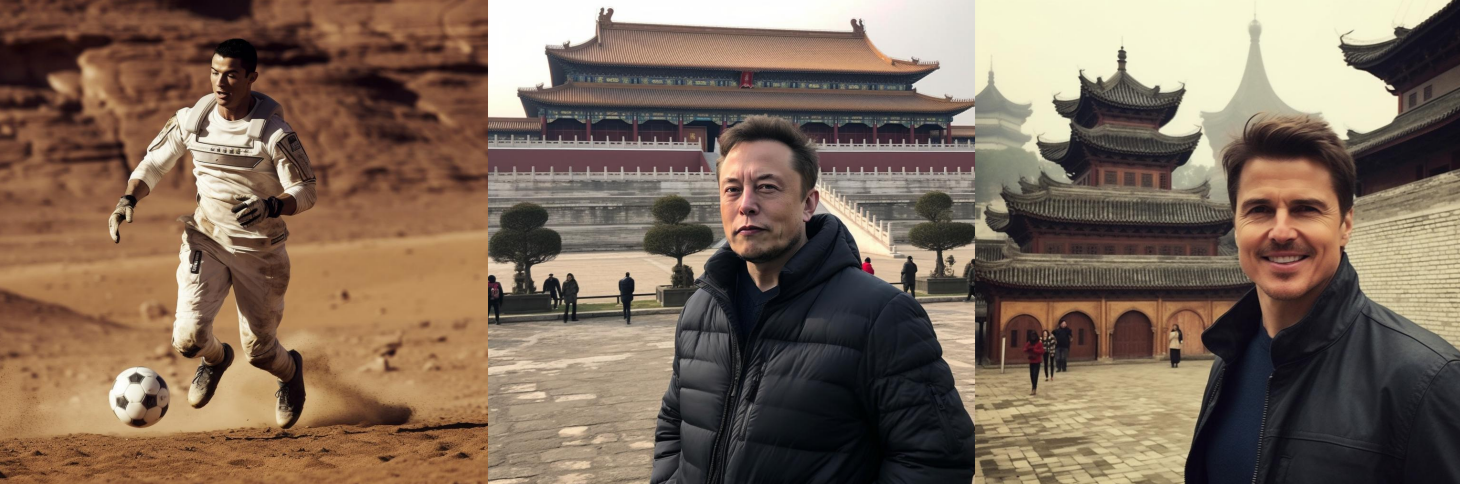
\includegraphics[width=0.8 \linewidth]{figures/ai_generated_images_from_seeing_is_not_believing.png} % Image filename
    \centering
    \caption{AI generated images \cite{lu2023seeingbelievingbenchmarkinghuman}} % Caption
    \label{fig:ai_generated_images} % Label
\end{figure}

This topic has been the focus of several recent studies. \cite{lu2023seeingbelievingbenchmarkinghuman} evaluates both human and AI capabilities in detecting fake images, and shows that humans are frequently misled by advanced image generation models. Although AI-based detection algorithms outperform humans, they still misclassify approximately 13\% of images. The study introduces the Fake2M dataset along with new benchmarking protocols, HPBench and MPBench, to support further research and improve the reliability of AI-generated content detection systems.

\cite{bird2023cifakeimageclassificationexplainable} presents a computer vision approach to distinguishing AI-generated images from real ones, utilising a synthetic dataset created with Latent Diffusion, classification via Convolutional Neural Networks, and interpretability through Grad-CAM. Achieving nearly 93\% accuracy, the study also introduces the CIFAKE dataset, a large collection of real and synthetic images, to support further research on the detection of AI-generated imagery.

This report aims to design and train a CNN (Convolutional Neural Network) to classify images as either AI generated or real. The trained model is then deployed to AWS SageMaker for inference and evaluated against comparable models. This work aims to contribute towards reliable detection methods that help distinguish AI generated content from real/handmade imagery, with the broader goal of supporting efforts to mitigate misinformation and related harms.
